\section{Testen}
In dit hoofdstuk komen er een aantal tests aanbod. deze tests zullen worden gebruikt om te controleren of de pH sensormodule aan de specificaties uit hoofdstuk \ref{sec:systemSpecifications} voldoet. Voor test 1 \& test 2 zijn de materialen uit \cref{tab:testMaterialen} gebruikt. Bij test 3 zijn de materialen uit ... gebruikt.
%Om de sensormodule te testen zijn een aantal materialen nodig. Deze materialen zijn gespecificeerd in \cref{tab:testMaterialen}.
\begin{table}[ht]
    \centering
    \begin{tabular}{l|l|l}
        Apparaat         & Serienummer & Beschrijving \\
        \hline
        MSREF1           & 23/RS03     & Referentie elektrode       \\
        MSFET 3330-2     & 23/205      & ISFET pH sensor            \\
        Tektronix MSO 46 & C019070     & Oscilloscoop               \\
        ISFETLezer       & 1           & ISFET uitlees schakeling   \\
        Harvester        & 1           & BMS en energy harvester    \\    
        \hline
    \end{tabular}
    \caption{Materialen die zijn gebruikt voor de tests}
    \label{tab:testMaterialen}
\end{table}

\subsection{Test 1}
De eerste test is bedoelt om te controleren of de uitgang van de opamp stabiel is. Dit is een belangrijke test om uit te voeren. Als de uitgang namelijk niet stabiel is, zal de spanning die de ADC uitleest niet goed overeen komen met de drempelspanning van de ISFET.

Om de test uit te voeren wordt de uitlees PCB verbonden met de voeding PCB, zodat de uitleesschakeling een voeding heeft. De probe van kanaal 1 van de oscilloscoop wordt verbonden met de uitgang van de opamp. De probe van kanaal 2 wordt verbonden met de drain van de ISFET. De ISFET wordt samen met de referentieelektrode in een pH7 bufferoplossing gestopt. De opstelling is in \cref{fig:test ISFET circuit best} schematisch te zien.

\begin{figure}[ht]
    \centering
    \def\svgwidth{0.75\textwidth}
    \input{img/ISFETCircuitBestTest.pdf_tex}
    \caption{De locatie van de scope probes in de schakeling om te testen of de uitgang stabiel is.}
    \label{fig:test ISFET circuit best}
\end{figure}


\subsubsection{Resultaten}

De eerste test resulteerde in een oscillerend signaal. De uitgang van de opamp gaf een signaal dat elke \qty{6.8}{\milli\second} pulseerde. Dit is te zien in \cref{fig:resultUgsUds}.
Een mogelijke reden hiervoor is dat de ISFET niet snel genoeg reageert op spanningsveranderingen tussen de gate (de referentie elektrode) en de source. Wanneer de opamp uitgang laag is, waardoor de gate-source spanning op de ISFET 0 V wordt, komt de drain-source spanning van de ISFET namelijk erg langzaam omhoog. Wanneer deze spanning boven de referentiespanning komt, gaat de uitgang van de opamp omhoog, waarna de drain-source spanning van de ISFET erg snel begint te dalen. Echter, wanneer de drain-source spanning vervolgens de referentiespanning bereikt, reageert de opamp hier merkwaardig genoeg niet direct op. De ingang van de opamp lijkt een hysterese werking te hebben. Dit zorgt voor een oscillerende werking. Ditzelfde resultaat kwam uit een andere test met een andere opmamp (de MCP6002).

Op de drain-source spanning is ook een tweede oscillatie met een hogere frequentie zichtbaar. Dit wordt waarschijnlijk veroorzaakt door de interne chopping van de gekozen opamp.


\begin{figure}[ht]
    \centering
    \def\svgwidth{0.75\textwidth}
    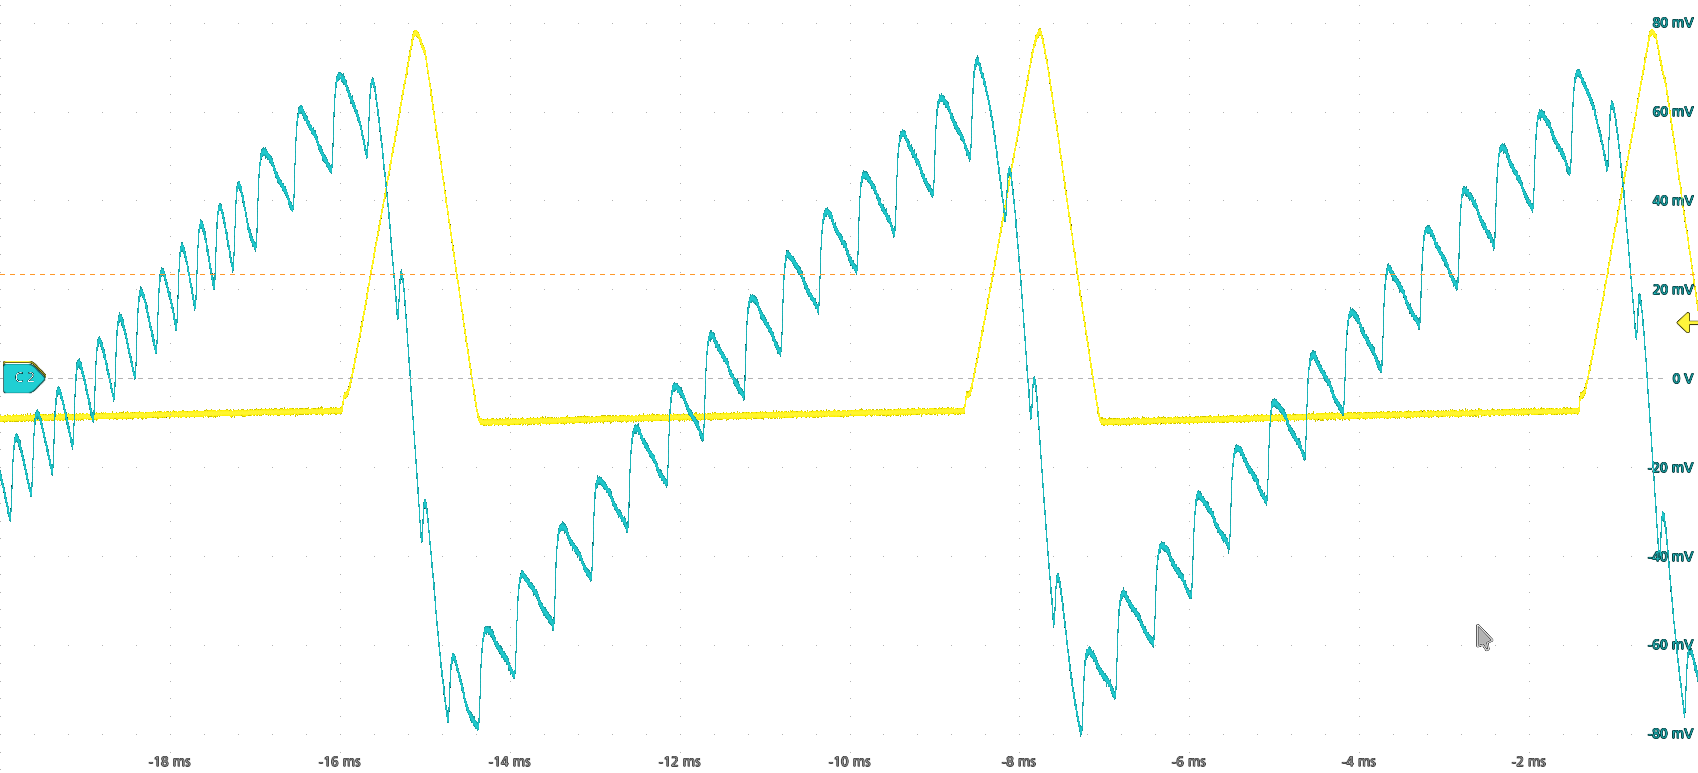
\includegraphics[width=0.8\textwidth]{testUgsUds.png}
    \caption{Het resultaat van de stabiliteitstest. Kanaal 1 (geel) is $U_{gs}$, kanaal 2 (lichtblauw) is $U_{ds}$.}
    \label{fig:resultUgsUds}
\end{figure}


\subsubsection{Discussie}
Er zijn meerdere mogelijke oplossingen voor de instabiliteit.
Eén mogelijke oplossing is een integrator plaatsen tussen de uitgang van de opamp en de gate van de ISFET. Dit zou ervoor zorgen dat de ISFET genoeg tijd heeft om te reageren op de veranderde gate-source spanning, waardoor deze de opamp kan bijhouden.

Een andere mogelijke oplossing is een RC-filter te plaatsen tussen de drain van de ISFET en de niet-inverterende ingang van de opamp. Dit zorgt ervoor dat de opamp trager gaat werken, waardoor de ISFET de opamp bij kan houden.

Er zal een aantal tests gedaan moeten worden om te vinden hoe de ISFET precies reageert op een verandering van de gate-source spanning, en hoe dit verschilt van een reguliere MOSFET. Zo kan een beter model opgesteld worden van de ISFET, waar dan vervolgens een betere uitleesschakeling mee ontworpen kan worden.


\subsection{Test 2} 
De volgende test is bedoelt om te testen of het uitgangssignaal verandert op basis van de pH waarde. 

Om te beginnen wordt de uitlees PCB verbonden met de voeding PCB, zodat de uitleesschakeling gevoed wordt. De probe van kanaal 1 van de oscilloscoop wordt verbonden met de ingang van de ADC. De probe van kanaal 2 wordt verbonden met de uitgang van de opamp. Vervolgens worden de ISFET en referentieelektrode in een pH7 bufferoplossing gestopt. De golfvorm die de oscilloscoop geeft kan nu worden opgeslagen. De meting wordt herhaalt met de ISFET en referentieelektrode in een pH4 bufferoplossing.

\subsubsection{Resultaten}
De resultaten van deze test zijn te zien in \cref{fig:resultspHMeasure}. Duidelijk is de amplitude van de uitgang van de opamp hoger op pH7 vergeleken met pH4.

\begin{figure}[ht]
    \centering
    \begin{subfigure}[b]{0.475\textwidth}
        \centering
        \def\svgwidth{\textwidth}
        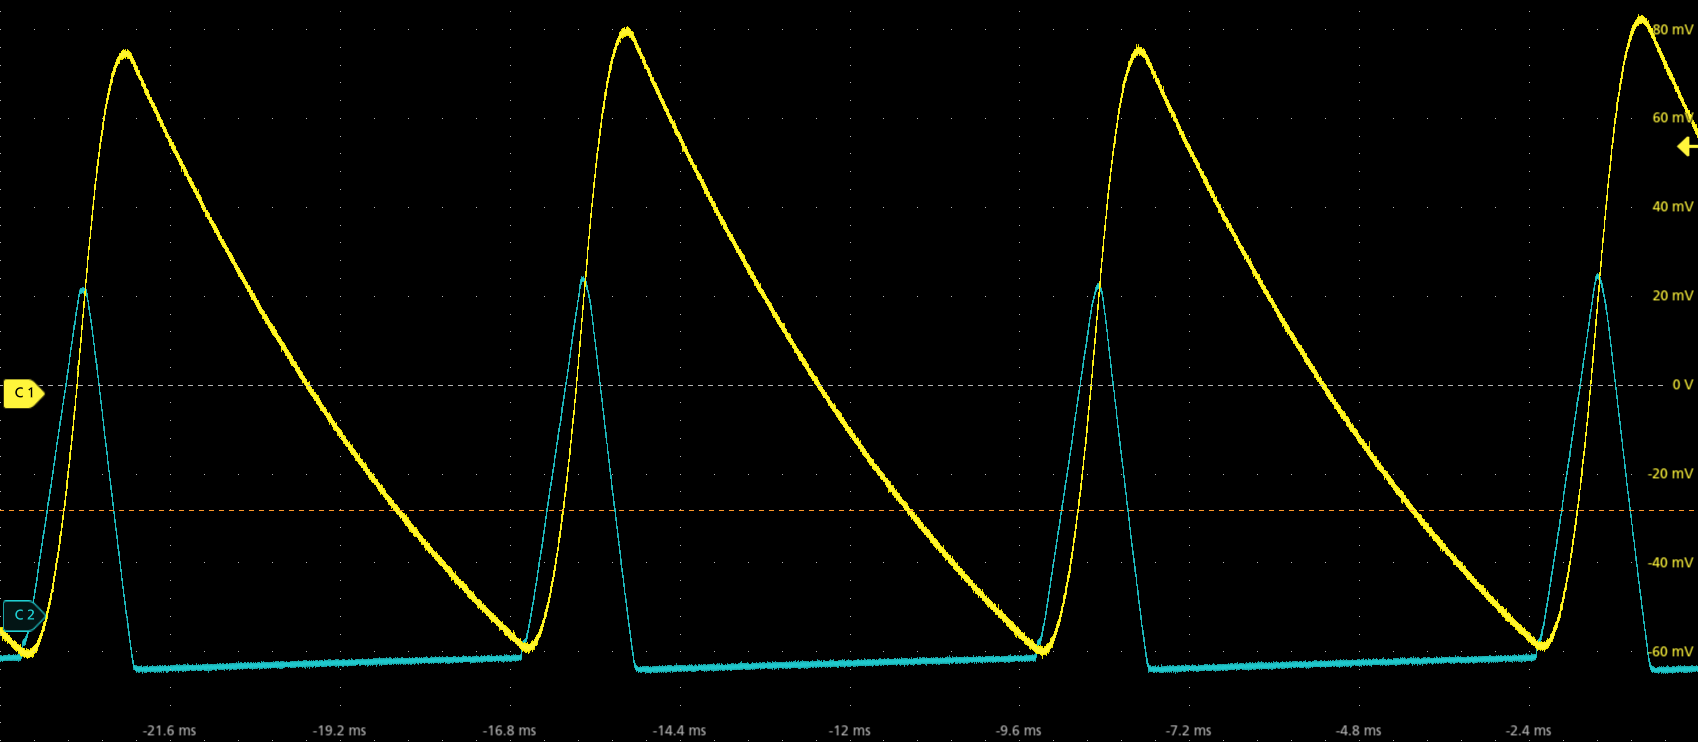
\includegraphics[width=\textwidth]{testpH7.png}
        \caption{De uitgang van de opamp (lichtblauw) en ingang van de ADC (geel) op pH7.}
        \label{fig:resultpH7}
    \end{subfigure}
    \hfill
    \begin{subfigure}[b]{0.475\textwidth}
        \centering
        \def\svgwidth{\textwidth}
        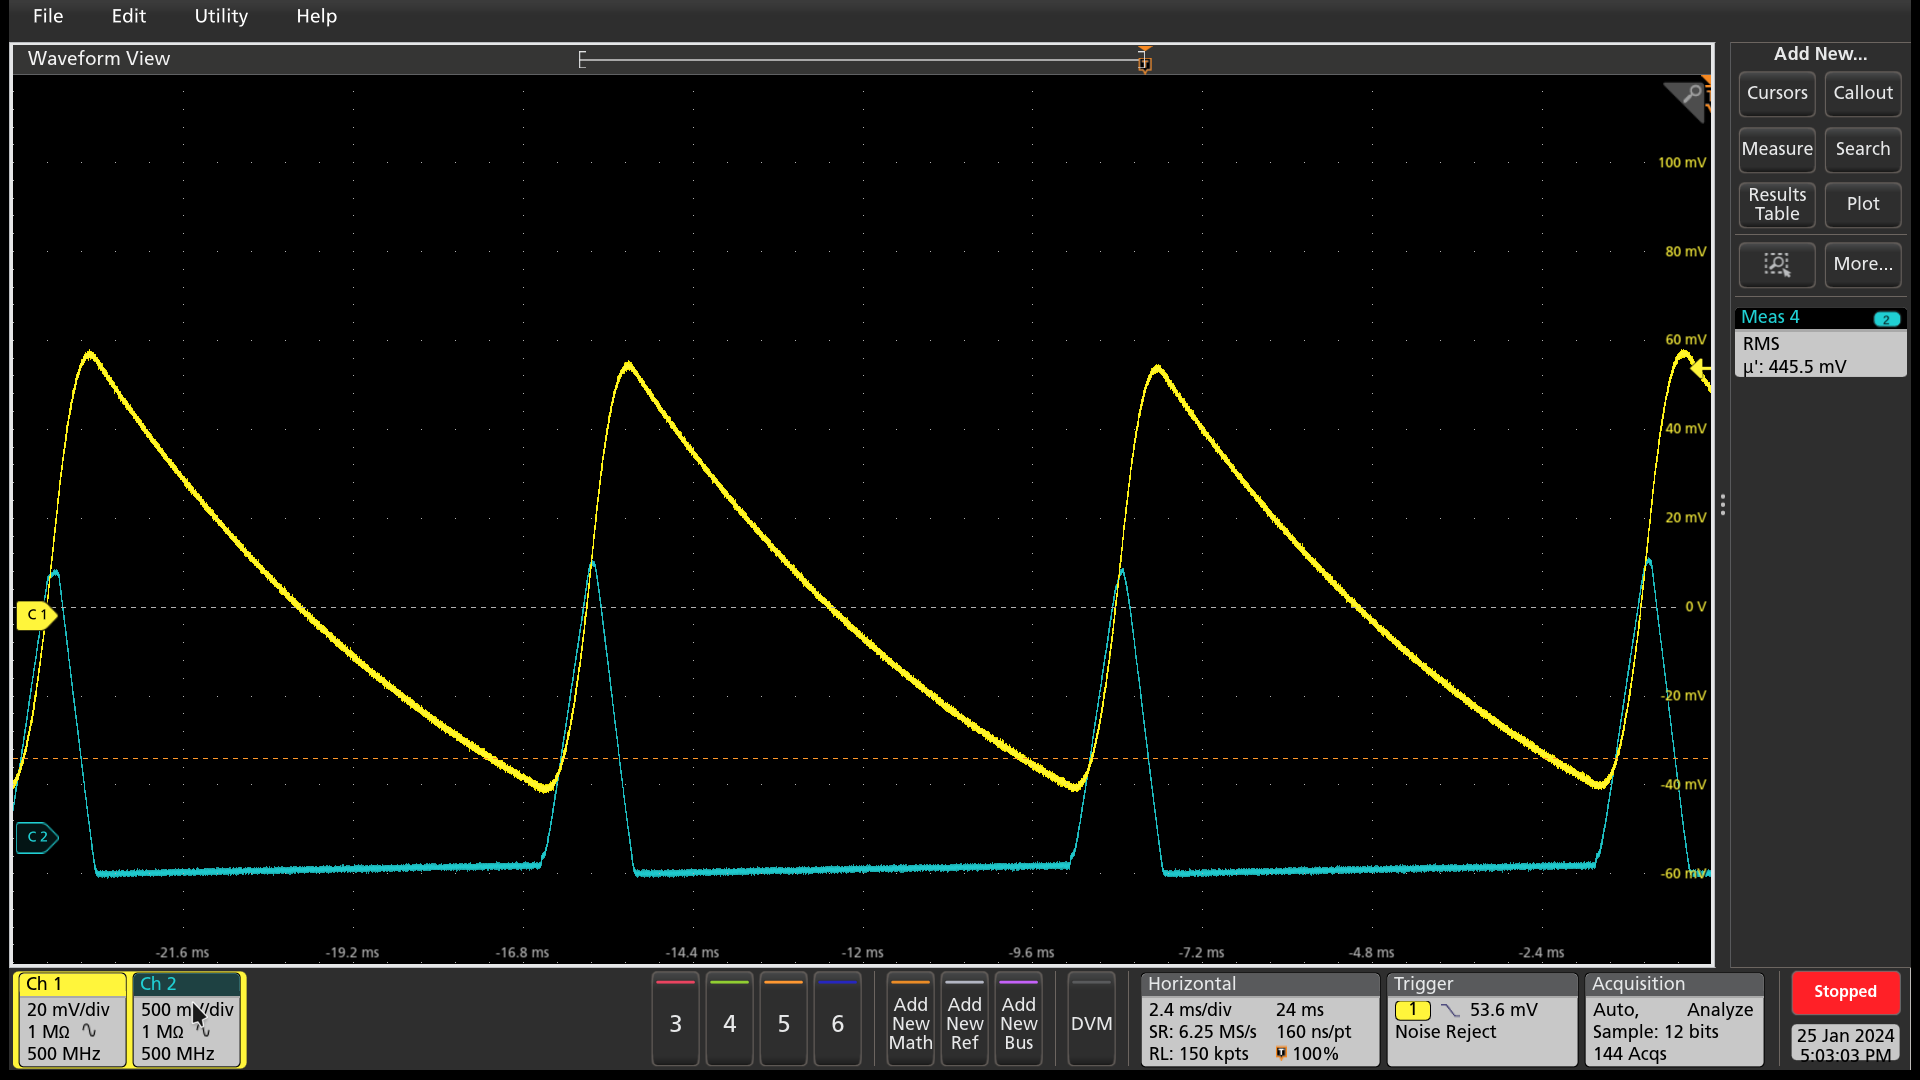
\includegraphics[width=\textwidth]{testpH4.png}
        \caption{De uitgang van de opamp (lichtblauw) en ingang van de ADC (geel) op pH4.}
        \label{fig:resultpH4}
    \end{subfigure}
    \caption{De uitgang van de meetschakeling op pH4 en pH7. Beide metingen hebben dezelfde schaal.}
    \label{fig:resultspHMeasure}
\end{figure}

\subsubsection{Discussie}
Een verandering van pH waarde heeft duidelijk een effect op het uitgangssignaal. Er kan echter nog weinig gezegd worden over de lineariteit van de uitgang op basis van de pH waarde. Hiervoor zou de uitgang eerst stabiel gemaakt moeten worden.
